\chapter{Faculty Workload Model}

\section{Introduction}

In an academic institution, teaching only constitutes a part of the overall workload of faculty members. They are also expected to perform research, manage research staff, supervise final-year projects, serve on peer review committees, and perform other administrative duties for the institution. Thus, to equitably allocate the teaching workload to faculty members, it is important to take the research and service contributions of the faculty into account.

The research workload of the faculty has typically been measured in terms of the number of research papers that the faculty has published \cite{finlay1994management, narasimhan32trase}. However, it was found to be a trailing indicator of the research workload of the faculty, being non-indicative of the research workload for the upcoming semester, while also being susceptible to abuse. This work proposes a new method to quantify the research workload of the faculty using the number of research staff that the faculty is supervising.

Additionally, it proposes a method to quantify the service workload of the faculty using the service duties that the faculty is performing. Using these, the research proposes a workload model that provides an accurate of the faculty workload in various domains, which is useful for the management to gain a better understanding of the workload of the faculty. This workload model also serves as the basis for the lecture allocation problem, where it establishes the limits for the teaching workload of the faculty to ensure that the faculty are not overloaded with work.

In the following sections, the various components of faculty workload are identified. Then, the technique of quantifying the research workload and service workload is described, which is followed by the description of the faculty workload model based on the research and service workload. Finally, the equitable teaching workload of the faculty is derived from the faculty workload model, and demonstrated with real-world faculty data.

\section{Components of Faculty Workload}

A faculty member's workload consists of multiple responsibilities and activities. These responsibilities and activities can be broadly classified into three categories:

\begin{enumerate}
  \item \textbf{Research Workload}

        This refers to the various research activities that the faculty performs. This includes supervision of research staff like post-doctoral fellows and research assistants, contributions towards research publications, acquiring research funding. These activities lead to the creation of new knowledge and the advancement of the research community. The research workload of a faculty member is quantified in \autoref{sec:modelling_research_workload}.

  \item \textbf{Teaching Workload}

        A faculty member's teaching workload consists of the activities that they perform towards the learning of their students. This can further be classified into two categories:

        \begin{enumerate}
          \item Formal Teaching

                This refers to the delivery of lectures, tutorials and labs to the students, and other activities that are directly related to the delivery of the course like preparation of course materials, setting and marking of assignments and examinations, and consultation with students. This part of the teaching workload was described in \autoref{ch:teaching_workload}.

          \item Informal Teaching

                This refers to the supervision of students outside of the formal teaching environment. This includes the supervision of Final-Year Projects (FYPs), Undergraduate Research Experience on Campus (URECA) projects and postgraduate students' research projects.

        \end{enumerate}

  \item \textbf{Service Workload}

        A faculty member's service workload consists of the various service activities that they perform. This includes departmental service - the various service activities that the faculty performs for the department, administrative duties - the various administrative duties that the faculty performs for the institution, and research service duties - the various service activities that the faculty performs for the research community. The service workload of a faculty member is quantified in \autoref{sec:modelling_service_workload}.

\end{enumerate}

\section{Modelling Faculty Workload}

The aim of the faculty workload model is to provide a simplified and accurate picture of the workload of the faculty, providing meaningful insights to the faculty and administration about how the workload of the faculty is distributed across the various activities and how it compares to the workload of other faculty. This is important as the workload of the faculty influences the distribution of teaching workload to the faculty, and the allocation of resources to the various departments. An inaccurate workload allocation model will result in an unfair distribution of workload and resources.

To guide the development of the faculty workload model, a set of objectives and principles were defined. These objectives and principles were used to guide the development of the faculty workload model, and ensure that the faculty workload model is able to achieve its objectives. The faculty workload model was then defined as a set of equations that quantifies the workload of the faculty across the various activities. This allowed the distribution of teaching workload to the faculty to be derived from the workload of the faculty across the various activities.

\subsection{Principles Guiding the Faculty Workload Model}
\label{sec:principles_guiding_workload_allocation_model}

To achieve the objectives of the workload allocation model, it is important to define a set of principles and attributes that the workload allocation model should satisfy. These principles and attributes are:

\begin{enumerate}

  \item \textbf{The workload allocation model should be consistent.}

        The workload allocation model should be able to consistently quantify the workload of various faculty. This is important as the workload allocation model will influence the distribution of teaching workload to the faculty, and the allocation of resources to the various departments. An inaccurate workload allocation model will result in an unfair distribution of workload and resources.

  \item \textbf{The workload allocation model should be transparent and easily understood.}

        Complexity is the enemy of transparency. A complex workload allocation model might be able to accurately quantify the workload of the various activities, but it will be difficult for the faculty to understand how the workload is being allocated. This causes the faculty to lose confidence in the workload allocation model, and will result in a lack of buy-in from the faculty. Additionally, a complex workload allocation model will be difficult to fine-tune and adapt to the needs of the institution.

  \item \textbf{The workload allocation model should be flexible and adaptable to the needs of the institution.}

        Carrying on from the previous point, the workload allocation model should be flexible and adaptable to the needs of the institution. Different institutions have different priorities and needs, and the workload allocation model should be able to adapt to these needs. For example, a teaching-focused institution might want to place more emphasis on teaching workload, while a research-focused institution might want to place more emphasis on research workload. The workload allocation model should be able to adapt to these different needs.

  \item \textbf{The workload allocation model should account for the zero-sum nature of workload.}

        The working hours of a faculty member are finite. As such, the workload of the various activities are zero-sum in nature. For example, a faculty member who spends more time on teaching will have less time to spend on research. The workload allocation model should account for this zero-sum nature of workload. This is important as the workload allocation model will influence the distribution of teaching workload to the faculty, and the allocation of resources to the various departments. An inaccurate workload allocation model will result in an unfair distribution of workload and resources.

  \item \textbf{The workload allocation model should be inclusive and account for the contributions of all faculty members.}

        An academic institution is made up of faculty members of different roles and seniority. The faculty are also broadly classified into lecturers and professors and the institution's goals and priorities for the faculty are influenced by the faculty's role and seniority. For example, a lecturer would be expected to spend more time on teaching than research, while a professor would be expected to make significant research and service contributions. The workload allocation model should be able to account for the contributions of all faculty members, regardless of their roles and seniority.

\end{enumerate}

\subsection{Designing a holistic faculty workload model}

In the absence of overtime, it is fair to assume that the total workload of a faculty should be closely comparable since the faculty are expected to have the same number of working hours, self-allocating any extra time towards research. Thus, the faculty workload model serves greater value in showing the comparative distribution of the workload of various faculty, and the corresponding distribution of their workload across teaching, research and service.

Instead of trying to quantify the workload of the faculty in terms of the number of hours, the ratio of the workload of the faculty across the various activities is quantified. To achieve this, the \textbf{RTS model} for faculty workload was defined as:

\begin{equation*}
  \text{Faculty Workload} = R:T:S
\end{equation*}

where workload of a faculty is represented as a ratio of the workload of the faculty across Research ($R$), Service ($S$) and Teaching ($T$). This model follows the following principles:

\begin{enumerate}
  \item Workload is a zero sum game.

        The sum of the $R$, $T$ and $S$ ratios always adds up to 12. This is because the workload of the faculty is constant, and spending extra time on one activity will result in a reduction of time spent on the other activities. In other words, the workload of the faculty is a zero-sum game.

  \item Linear distribution of workload.

        Each activity is distributed linearly in the model. This means that if a faculty has twice the R-ratio in comparison to another faculty, they are expected to have double the research workload. This is to ensure that the model is easily understandable, and representative of the actual workload of the faculty.

  \item Each Activity has a minimum workload.

        The faculty is allocated a minimum of 2 units of workload for each of the activities. This is to ensure that the faculty are able to make meaningful contributions to the various activities. This also means that each activity has a maximum workload of 8 units, since the sum of the $R$, $T$ and $S$ ratios always adds up to 12.

\end{enumerate}

This RTS model serves not only as a method to quantify the workload of the faculty, but it also serves as a method to distribute the workload. In the scope of this project, since the focus is on the teaching workload of the faculty, the RTS model is used to quantify the research and service workload of the faculty, and accordingly distribute the teaching workload of the faculty as shown in the following sections.


\section{Modelling Research Workload}
\label{sec:modelling_research_workload}

\subsection{Strategies to Quantify Research Workload}

A comprehensive measurement of research workload would require the quantification of the various research activities that the faculty performs. However, the individual research activities are not easily quantifiable. For example, even though we know the number of research papers that the faculty has published, the effort that goes into publishing each research paper can vary greatly depending on the topic of the research paper, the field of study, the quality of the research paper etc. Additionally, measuring at a low level of granularity would result in a large number of error sources, and would also be difficult to fine-tune and adapt to the needs of the institution.

As we we defined in \autoref{sec:principles_guiding_workload_allocation_model}, the workload allocation model should be transparent and easily understood. Thus, a simple and transparent method to quantify the research workload of the faculty is to find an activity that is representative of the entirety of the research workload. This activity should be easily quantifiable, and should be a leading indicator of the research workload of the faculty.


\subsubsection{Research Publication}

Research publication involves performing academic research and publishing the results of the research in conferences and journals. This is one of the most important activities of a faculty member, as it leads to the creation of new knowledge and the advancement of the research community. The workload of research publication is dependent on the number of research papers that the faculty has published, as well as the quality and subject matter of the research papers. For example, a faculty member who has published a research paper in a top-tier conference would generally be expected to have a higher research publication workload than a faculty member who has published a research paper in a lower-tier conference.

However, the research publication workload is difficult to quantify due to the difference in the quality of research, the subject matter of the research papers, as well as the variations in the research publication venues. Moreover, research papers are only published after the research has been completed which makes them a trailing indicator of research publication workload, being able to quantify the research publication workload of the previous semesters, but not the upcoming semester. This makes the research publication workload unsuitable as a measure of the overall research workload of the faculty.

\subsubsection{Research Funding}

Acquiring research funding from external sources involves the writing of research proposals, as well as the application and management of research grants. Different research grants have different levels of complexity and scrutiny in their application process. The research funding may be measured on the basis of the total amount of research funding that the faculty has acquired. The number of research grants that a faculty has acquired or applied to can also be used as a measure of the research funding.

However, this is not an accurate reflection of the total research workload as the amount of research funding that a faculty has acquired as it doesn't directly correlate to the amount of research the faculty has performed. It also doesn't directly correlate to the amount of research staff supervision workload that the faculty has, as the research funding may be used to buy lab equipment, etc. Additionally, research funding is not spent immediately, and may be spent over a period of multiple years. This makes the research funding workload a leading indicator, but the period that the research funding is representative of is not known. Due to these factors, the research funding workload is not suitable as a measure of the overall research workload of the faculty.

\subsubsection{Research Staff Supervision}

Research Staff Supervision refers to the supervision of post-doctoral fellows, research fellows and research assistants. This is one of the most important activities of a faculty member, as most of the research is conducted in collaboration with the research staff that they are supervising. The research staff supervision workload is dependent on the number of research staff that the faculty is supervising, as well as the seniority of the research staff. For example, a faculty member who is supervising a post-doctoral fellow would be expected to spend less time on research supervision than a faculty member who is supervising a research assistant, as the post-doctoral fellow would be expected to be more independent than the research assistant.

The staff supervision workload was found to be a leading indicator of the research publication workload of the faculty. This is because for a faculty, the research is largely conducted in collaboration with the research staff that they are supervising. It is also indicative of the number of future publications that the faculty will be able to author or co-author. Thus, the research staff supervision workload can be used as a proxy for the research publication workload of the faculty. The research publication workload was found to be directly proportional to the research staff supervision workload of the faculty.

Similar to the publication workload, the research funding workload was also found to be directly proportional to the research staff supervision workload of the faculty. This is because the number of research staff that the faculty can hire is dependent on the amount of research funding that the faculty has acquired. Additionally, the assistance of the research staff is also required in the application of research grants. Thus, the research staff supervision workload can be used as a proxy for the research funding workload of the faculty.

The research staff supervision workload was thus found to be a representative indicator of the total research workload of the faculty.

% Additionally, another component of research workload is the research service workload. This includes the service activities that the faculty performs for the research community. For example, the faculty might be serving on the program committee of a conference, or the editorial board of a journal, or might be reviewing research papers for conferences and journals. The workload of research service is dependent on the number of research service activities that the faculty is performing, as well as the seniority of the research service activities. However, this activity is classified as service workload and is not considered as part of the research workload.

\subsection{Calculating Research Workload}
\label{sec:calculating_research_workload}

% Thus, the research workload of a faculty can be written as a function of the research staff supervision workload of the faculty. The research workload of a faculty can be quantified using the following formula:

% \begin{equation*}
%   R = N_{PD} +  N_{RA}
% \end{equation*}

% where $N_{PD}$ is the number of post-doctoral fellows that the faculty is supervising, and $N_{RA}$ is the number of research assistants that the faculty is supervising.

% This has the advantage of being a simple workload allocation model that is easy to understand and fine-tune, as the only parameter that needs to be tuned is the workload of supervising a post-doctoral fellow relative to the workload of supervising a research assistant. Additionally, this is also a leading indicator of the total research workload of the faculty for the upcoming semester.

% \subsection{Addressing Hierarchy Effects in Research}

As described above, quantifying the research workload of a faculty as a function of the research staff working under them has considerable advantages. A simple linear function can be used to quantify the research workload of a faculty. However, one key observation from how faculty supervise a large cohort of research staff was that the faculty do not directly supervise all of the research staff. Instead, the faculty supervise a small number of senior research staff, who in turn supervise a larger number of junior research staff. This not only reduces the workload of the faculty, but also provides a career progression path for the research staff and an opportunity for the senior research staff to gain supervisory experience. To account for this hierarchy effect, a non-linear function can be used to quantify the research workload of a faculty. The non-linear function is expected to have the following properties:

\begin{enumerate}

  \item The research workload of a faculty should be a monotonically increasing function of the number of research staff that they are supervising
  \item The research workload of a faculty should rise linearly for a small number of research staff, and then rise non-linearly for a large number of research staff to account for the hierarchy effect
  \item The research workload of a faculty should asymptotically approach a maximum value as beyond a certain number of research staff, the research workload of the faculty will not increase significantly

\end{enumerate}

The non-linear function that satisfies the above properties is the hyperbolic tangent function, which is defined as:

\begin{equation*}
  \tanh(x) = \frac{e^{2x} - 1}{e^{2x} + 1}
\end{equation*}

where $L$ is the maximum value of the function, $k$ is the steepness of the curve, and $x_0$ is the midpoint of the curve where the function increases linearly. The hyperbolic tangent function is plotted in \autoref{fig:tanh_full_function}.

\begin{figure}[htpb]
  \centering
  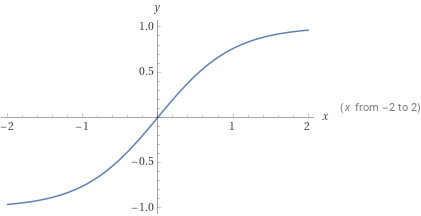
\includegraphics[width=0.5\linewidth]{images/tanh_fullplot.png}
  \caption{\(\tanh(x)\) for \(x \in [-2, 2]\)}
  \label{fig:tanh_full_function}
\end{figure}

We're only interested in the positive half of the hyperbolic tangent function, which has a constant slope for $x \to 0$, and is asymptotic to 1 as $x \to \infty$. The positive half of the hyperbolic tangent function is plotted in \autoref{fig:tanh_function}.

\begin{figure}[htpb]
  \centering
  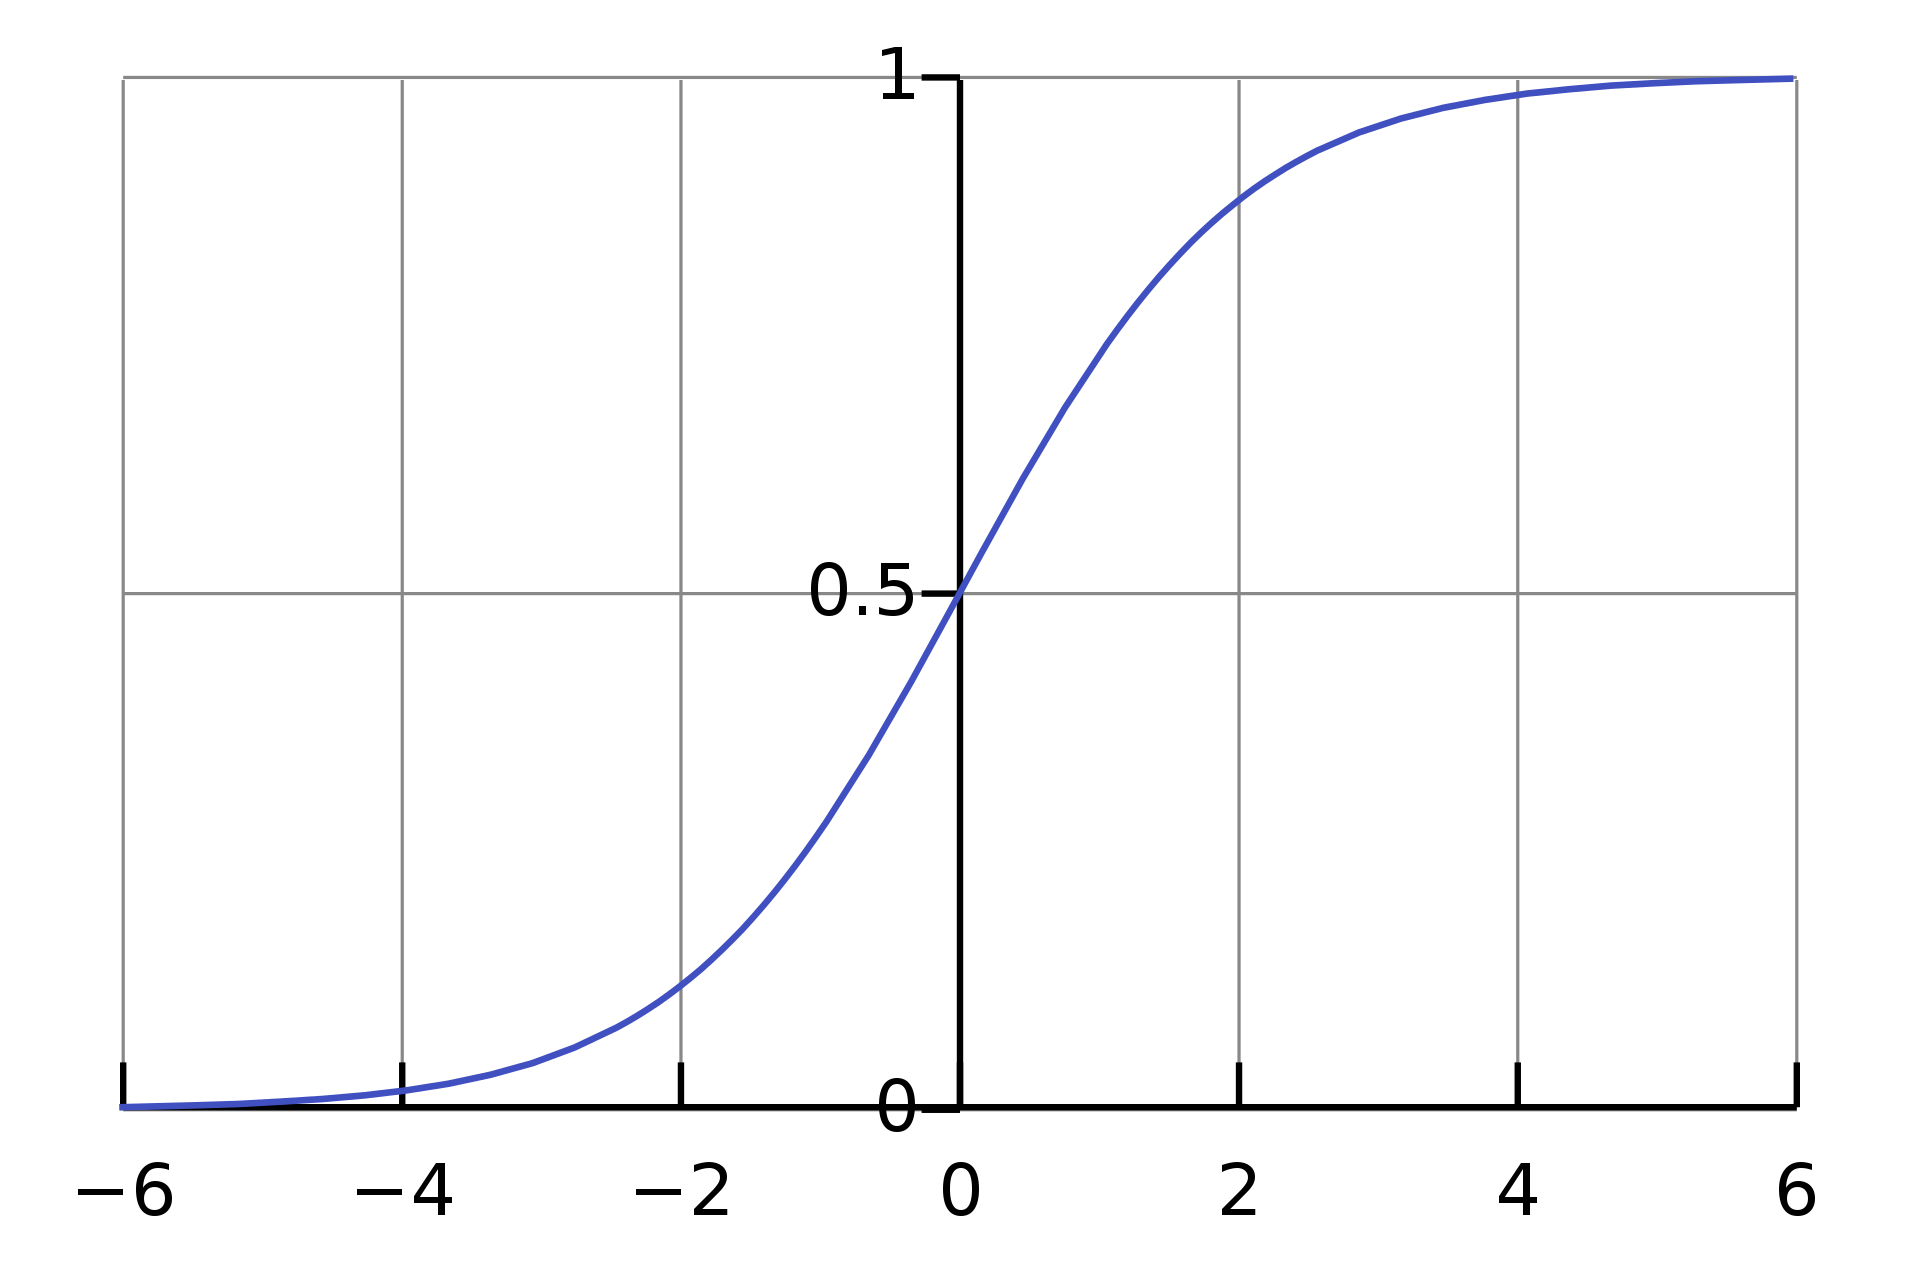
\includegraphics[width=0.5\linewidth]{images/tanh_plot.png}
  \caption{\(\tanh(x)\) for \(x \in [0, 4]\)}
  \label{fig:tanh_function}
\end{figure}


It was found that due to the hierarchical nature of research staff management, the research staff supervision workload can be modelled using a hyperbolic tangent function has a range of $[0, 1]$. Since it is known that the range of the research workload is between 2 and 8, i.e. a range of 6 units, the research workload is rescaled to have a range of $[2, 8]$. The steepness of the curve was also tweaked so that the research workload so that the research workload approaches the maxima at around 10 research staff. This results in the following formula:

\begin{equation}
  R  = 2 + 6\ \tanh(x/6)
\end{equation}

where $x$ is the total number of research staff members that the faculty is supervising. Individual research staff seniority was not taken into account, since the hiring patterns of the faculty are such that a small number of senior research staff are hired, who in turn supervise a larger number of junior research staff.

\begin{figure}[H]
  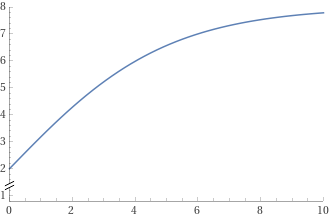
\includegraphics[width=0.5\textwidth]{images/rts_research_plot.png}
  \centering
  \caption{Research Workload ($R$)}
  \label{fig:rts_research_plot}
\end{figure}

\autoref{fig:rts_research_plot} shows the research workload of the faculty as a function of the number of research staff that the faculty is supervising. The research workload is a monotonically increasing function of the number of research staff that the faculty is supervising. The research workload rises linearly for a small number of research staff, and then rises non-linearly for a large number of research staff to account for the hierarchy effect. The research workload asymptotically approaches a maximum value of 8 as beyond a certain number of research staff, the research workload will not increase significantly.


\section{Modelling Service Workload}
\label{sec:modelling_service_workload}

The service workload of a faculty consists of the various service activities that they perform. The service activities of a faculty include but are not limited to the following:

\begin{enumerate}

  \item \textbf{Departmental Service}

        This is the various service activities that the faculty performs for the department. It includes serving on departmental committees, as well as performing administrative duties for the department.

  \item \textbf{Administrative Duties}

        This is the various administrative duties that the faculty performs for the institution. It includes duties like serving on various committees and panels the admissions panel, the scholarship review panel and the examinations committee, coordinating a research center etc.

  \item \textbf{Research Service Duties}

        This is the various service activities that the faculty performs for the research community. It includes serving on the program committee of a conference, or the editorial board of a journal, or reviewing research papers for conferences and journals.

\end{enumerate}

The service workload of a faculty is dependent on the number of service duties that the faculty is performing, as well as the amount of effort required to perform each of these duties. Since the nature of each service duty is different, it is difficult to quantify the service workload of a faculty through a heuristic approach. Instead, a simple weighted average of the service workload of each of these duties can be used, where the weights correspond to the workload per semester for each of these duties. The service workload of a faculty can be quantified using the following formula:

\begin{equation*}
  \text{Service Workload} = \sum_{i=1}^{N_{sd}} w_i
\end{equation*}

where $N_{sd}$ is the number of service duties that the faculty is performing, and $w_i$ is the workload per semester of the $i$-th service duty.

Some of the service duties are performed by all faculty members. For example, all faculty members are expected to perform some research service duties, be it reviewing research papers or serving on the program committee of a conference. These service duties are excluded from the workload allocation model as they are not indicative of the workload of an individual faculty member. The allocation of service duties also depends on the seniority of the faculty member. For example, a junior faculty member would be expected to generally perform less service duties and contribute primarily towards teaching and research, while as the faculty member progresses in their career, they would be expected to perform more service duties like serving on departmental committees and major administrative duties like coordinating a research center, or even serving as the Chair of the department. A typical faculty member would be expected to perform 0-2 service duties per semester, while senior faculty members would be expected to perform 2-4 service duties per semester.

Some of the service duties and their corresponding workload per semester are shown in \autoref{tab:service_duties}.

\begin{table}[htpb]
  \centering
  \begin{tabular}{|l | l | r |}
    \hline
    Designation     & Service Duty                                  & Workload \\
    \hline
    Member          & Industrial Attachment Steering Committee      & 1.00     \\
    Member          & Research Mentorship and Consultancy Committee & 1.00     \\
    Member          & Nanyang Research Programme Committee          & 1.00     \\
    Coordinator     & Final Year Projects                           & 1.00     \\
    Director        & Research Centre                               & 1.00     \\
    Group Lead      & Research Focus Group                          & 1.25     \\
    Member          & Research Integrity Committee                  & 1.00     \\
    Member          & Scholarship Interview Panel                   & 1.00     \\
    Member          & School Review Committee                       & 1.00     \\
    Member          & School Reappointment Committee                & 1.00     \\
    Member          & School Search Committee                       & 1.00     \\
    Chairperson     & Student Outreach Committee                    & 1.25     \\
    Coordinator     & Time-Tabling                                  & 1.00     \\
    Associate Chair & Associate Chair                               & 1.00     \\
    \hline
  \end{tabular}
  \caption{An example of how service duties and workload can be framed}
  \label{tab:service_duties}
\end{table}


It was found that each of the service duties has a particular impact on the workload of the faculty. For example, serving on the Industrial Attachment Steering Committee has an impact of 1 unit. In addition, even if the faculty is not performing any service duties, they are still expected to perform a minimum of 2 units of service workload. Thus, the service workload of the faculty can be quantified using the following formula:

\begin{equation}
  S = 2 + \sum_{i=1}^{N_{sd}} w_i
\end{equation}

where $N_{sd}$ is the number of service duties that the faculty is performing, and $w_i$ is the workload per semester of the $i$-th service duty.

A maximum cap of 8 units is also imposed on the service workload of the faculty, since the sum of the $R$, $T$ and $S$ ratios always adds up to 12. This means that a faculty will only be rewarded for their service duties up to a certain extent. This is to ensure that the faculty are able to make meaningful research and teaching contributions as well, and not be overloaded with service duties.

\section{Determining Equitable Teaching Workload}
\label{sec:determining_equitable_teaching_workload}

The service and research workload of the faculty are predictive, i.e. they are leading indicators of the workload of the faculty for the upcoming semester. The number of staff that the faculty is supervising is indicative of how much research workload will be involved, and the number of service duties that the faculty is performing for the semester is indicative of how much service workload will be involved.

While the research and service workload are pre-determined, we have the opportunity to use the teaching workload to balance the workload of the faculty. This allows the total workload of each faculty to be comparable, and ensures that the faculty are not overloaded with work. Thus, with the service and research workload of the faculty quantified, the teaching workload of the faculty can be derived from the RTS model. Since $R + T + S = 12$, the teaching workload of the faculty can be quantified using:

\begin{equation}
  T = 12 - R - S
\end{equation}

The teaching workload is also subject to the same minimum and maximum workload constraints as the research and service workload. This means that the teaching workload of the faculty is capped at a maximum of 8 units, and a minimum of 2 units. This is to ensure that the school is able to make use of their teaching expertise in their respective fields.


\begin{figure}[H]
  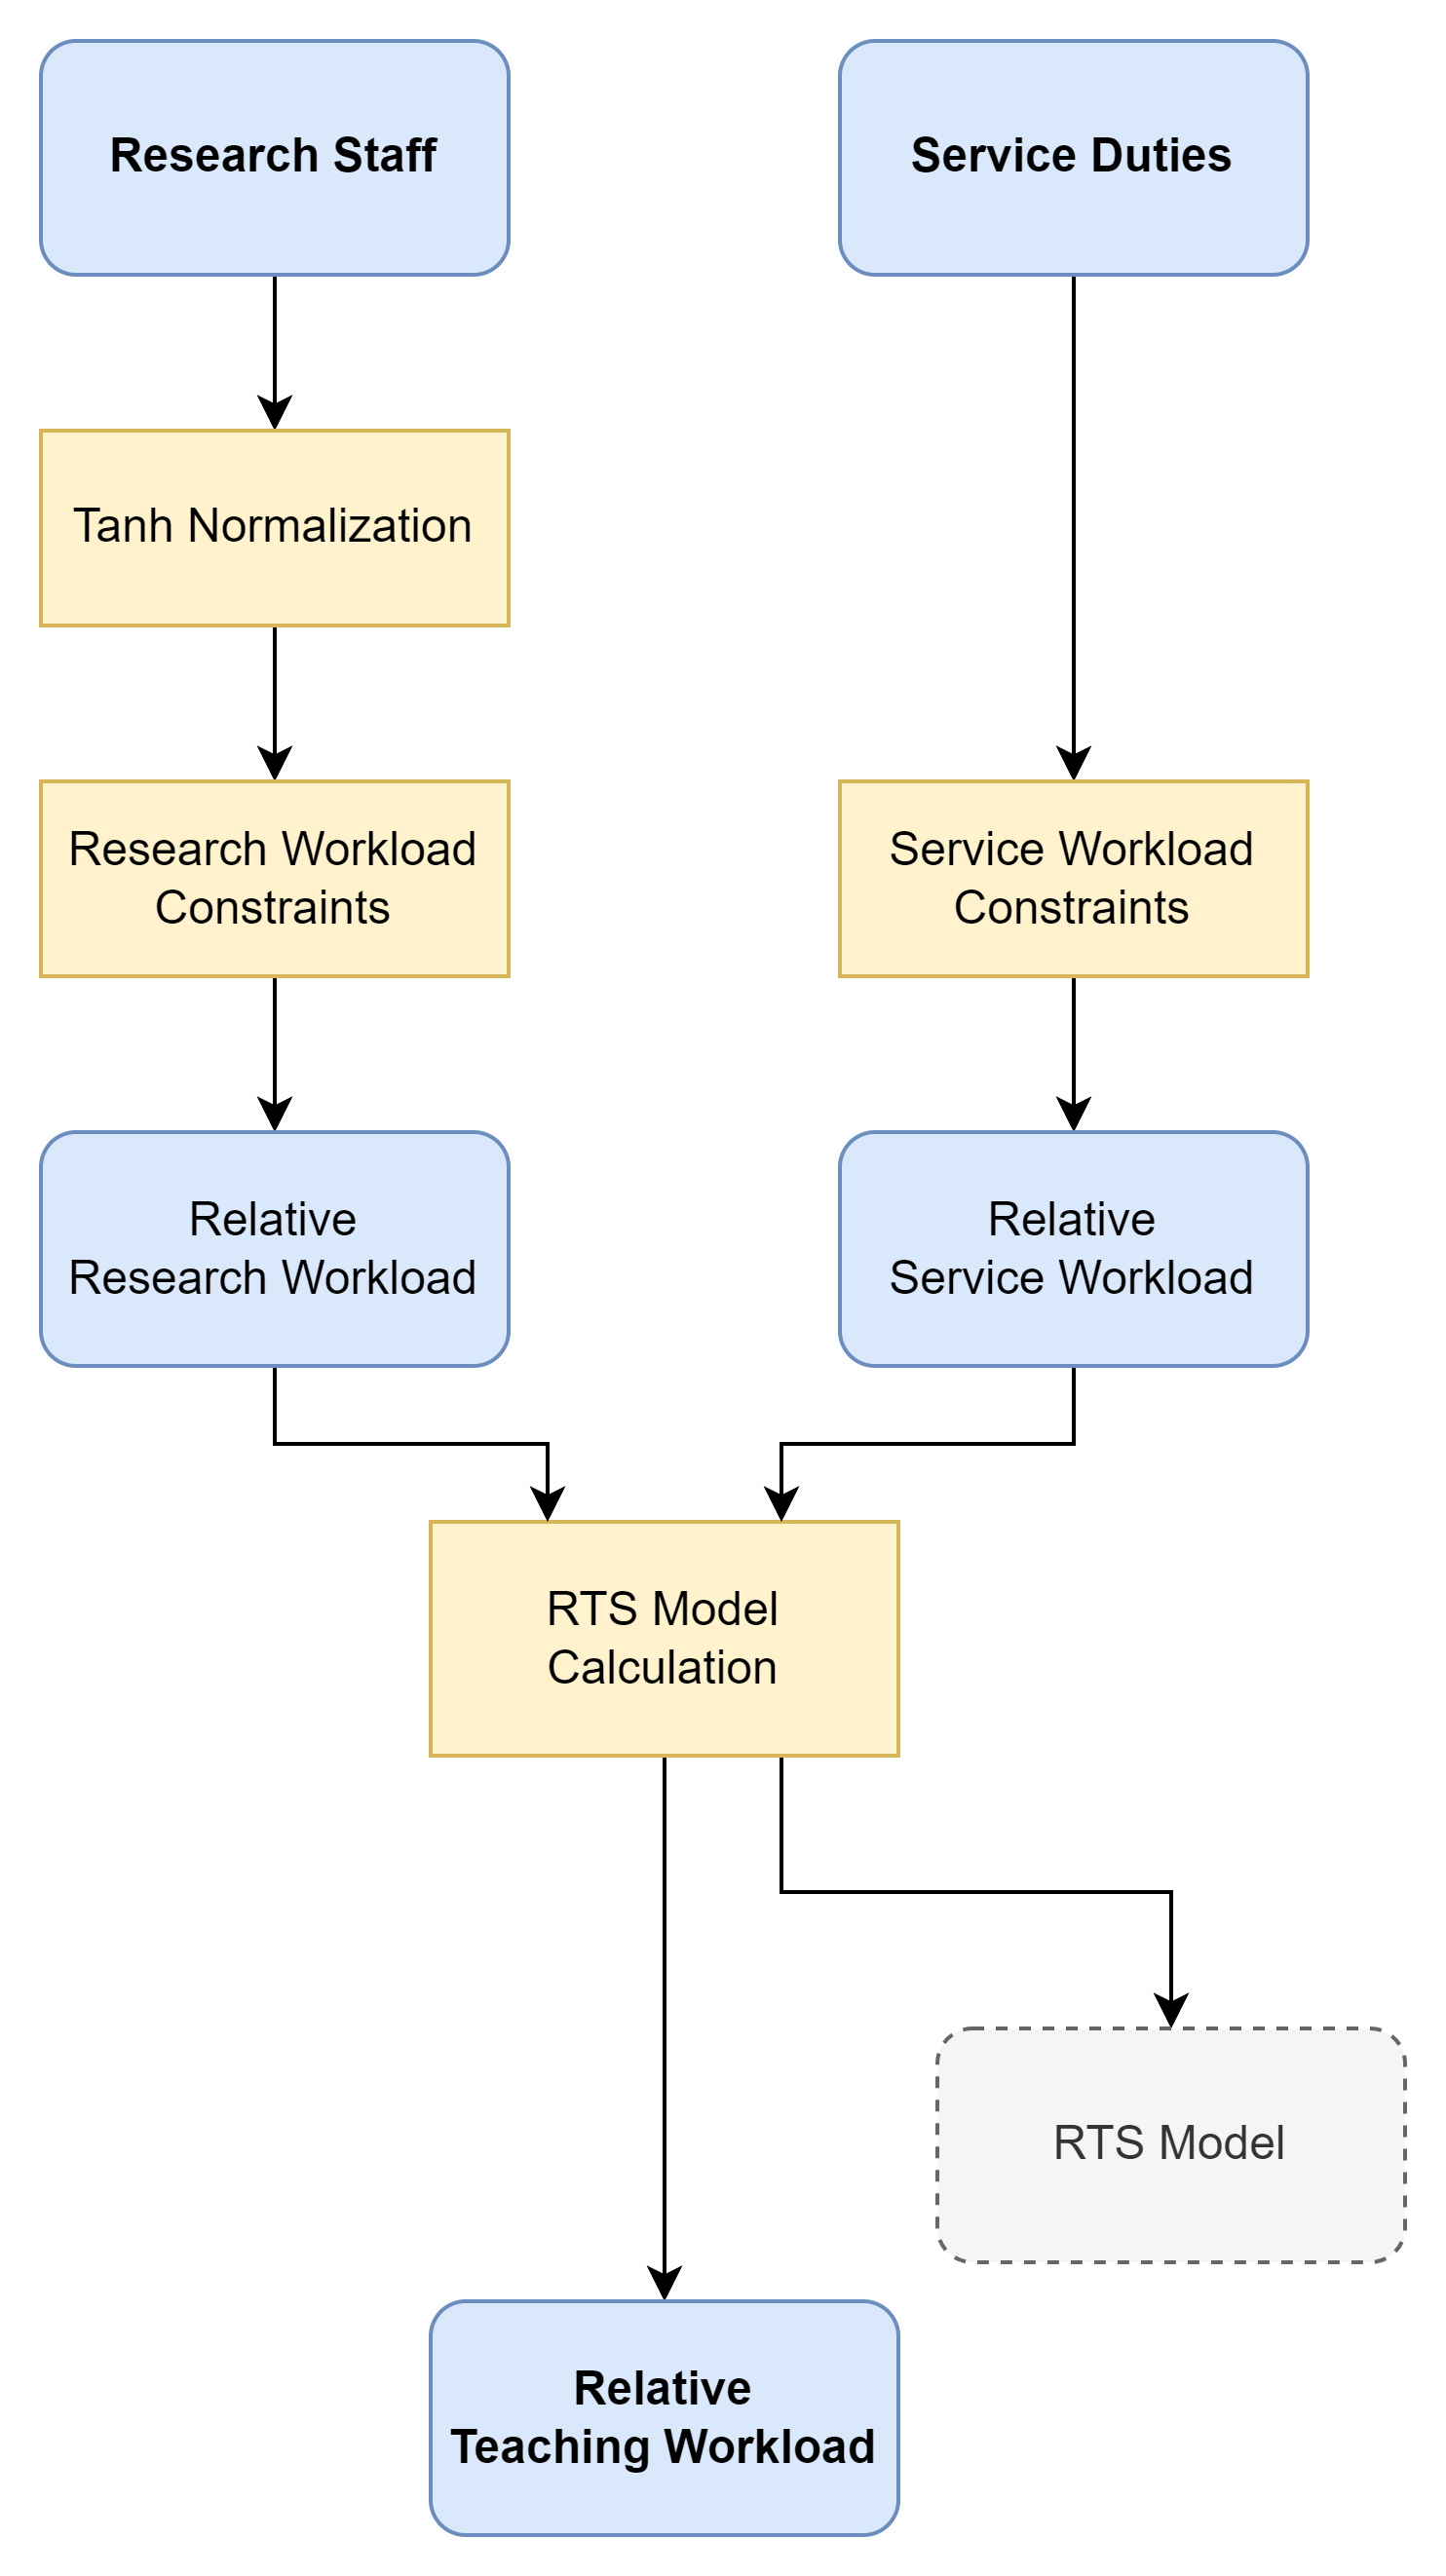
\includegraphics[width=0.5\textwidth]{images/faculty_wam.png}
  \centering
  \caption{Deriving Teaching Workload from RTS Model}
  \label{fig:faculty_wam}
\end{figure}


\section{Summary}

The RTS Model for faculty workload establishes a simple and transparent method to quantify and distributing the faculty workload in an equitable manner. This involves quantifying the research workload of the faculty as a function of the number of research staff that the faculty is supervising, and quantifying the service workload of the faculty as simple weighted increments for each of the service duties that the faculty is performing. This allows the teaching workload of the faculty to be derived from the RTS model, and ensures that the total workload of each faculty is comparable.

In the next chapter, the teaching workload derived using the RTS model will be used as the basis for the lecture allocation problem, where it will establish the limits for the teaching workload of the faculty to ensure that the faculty are not overloaded with work.
